\centerline{\bf \Huge Теорема Кадзи}

\begin{flushright}
        \scriptsize{Эпизод 16. Смертельная болезнь}
\end{flushright}

\problem{1}
Хорды $A C$ и $B D$ окружности $\Omega$ пересекаются в точке $X$. Докажите, что радикальная ось окружностей, вписанных в криволинейные треугольники $A X B$ и $C X D$, проходит через середины дуг $B C$ и $D A$.

\problem{2}
Пусть $\omega$ --- окружность с диаметром $A B$, а $P$ и $Q$ - две точки на $\omega$, лежащие по разные стороны от $A B$. Точка $T$ --- проекция точки $Q$ на $A B$. Пусть $\omega_1$ и $\omega_2$ - окружности с диаметрами $T A$ и $T B$ соответственно, а $P C$ и $P D$ --- отрезки касательных, проведённых из точки $P$ к окружностям $\omega_1$ и $\omega_2$ соответственно. Докажите, что $P C+P D=P Q.$

\problem{3}
Окружности $\omega_1, \omega_2$ касаются внешним образом в точке $I$, а также обе касаются внутренним образом некоторой окружности $\omega$. Внешняя касательная к $\omega_1$ и $\omega_2$ пересекает $\omega$ в точках $B$ и $C$, а общая касательная в точке $I$ - в точке $A$, по ту же сторону от $B C$, что и $I$. Докажите, что $I$ центр вписанной окружности треугольника $A B C$.

\problem{4}
В треугольнике $A B C$ на стороне $A C$ взята точка $D$. Рассмотрим окружность, касающуюся отрезка $A D$ в точке $M$, отрезка $B D$ и окружности, описанной около треугольника $A B C$. Докажите, что прямая, проходящая через $M$ параллельно $B D$, касается окружности, вписанной в треугольник $A B C$.

\problem{5}
В треугольнике $A B C$ пусть $\omega_A, \omega_B, \omega_C$ - окружности, касающиеся соответственно сторон $B C, C A, A B$ в их серединах и дуг $B C, C A, A B$ описанной окружности, не содержащих соответственно точек $A, B, C$. Если $\delta_{B C}, \delta_{C A}, \delta_{A B}$ обозначают длины общих внешних касательных между парами $\left(\omega_B, \omega_C\right),\left(\omega_C, \omega_A\right)$ и $\left(\omega_A, \omega_B\right)$, соответственно, докажите, что

$$
\delta_{B C}=\delta_{C A}=\delta_{A B}=\frac{a+b+c}{4} .
$$

\problem{6}
\textbf{Внешняя теорема Тебо}. Пусть $\triangle A B C$ - треугольник, пусть $(\omega, R)$ - его описанная окружность, и пусть $D$ - точка на $B C$, такая что $\angle B D A=\theta$ (см. Рис. 1). Пусть $\left(\omega_1, r_1\right)$ - окружность, касающаяся $B C$ или её продолжения в точке $P$, касающаяся $A D$ или её продолжения в точке $M$, а также касающаяся $\omega$ внешним образом. Пусть $\left(\omega_2, r_2\right)$ - окружность, касающаяся $B C$ или её продолжения в точке $Q$, касающаяся $A D$ или её продолжения в точке $N$, а также касающаяся $\omega$ внешним образом. 

\newpage

\hspace{3mm}

Пусть $\left(I_a, r_a\right)$ - вневписанная окружность треугольника $\triangle A B C$, касающаяся стороны $B C$ и сторон $A B, A C$ или их продолжений. Тогда:

(a) $r_a=r_1 \cos ^2(\theta / 2)+r_2 \sin ^2(\theta / 2)$.

(b) Прямые $l_1$ и $l_2$, проходящие через $P$ и $Q$ соответственно и параллельные $A D$, касаются вневписанной окружности $(I_a, r_a)$.

(c) $O_1, O_2$ и $I_a$ коллинеарны.

(d) $\frac{O_1 I_a}{O_2 I_a}=\tan ^2(\theta / 2)$.



\begin{figure}[h]
    \centering
    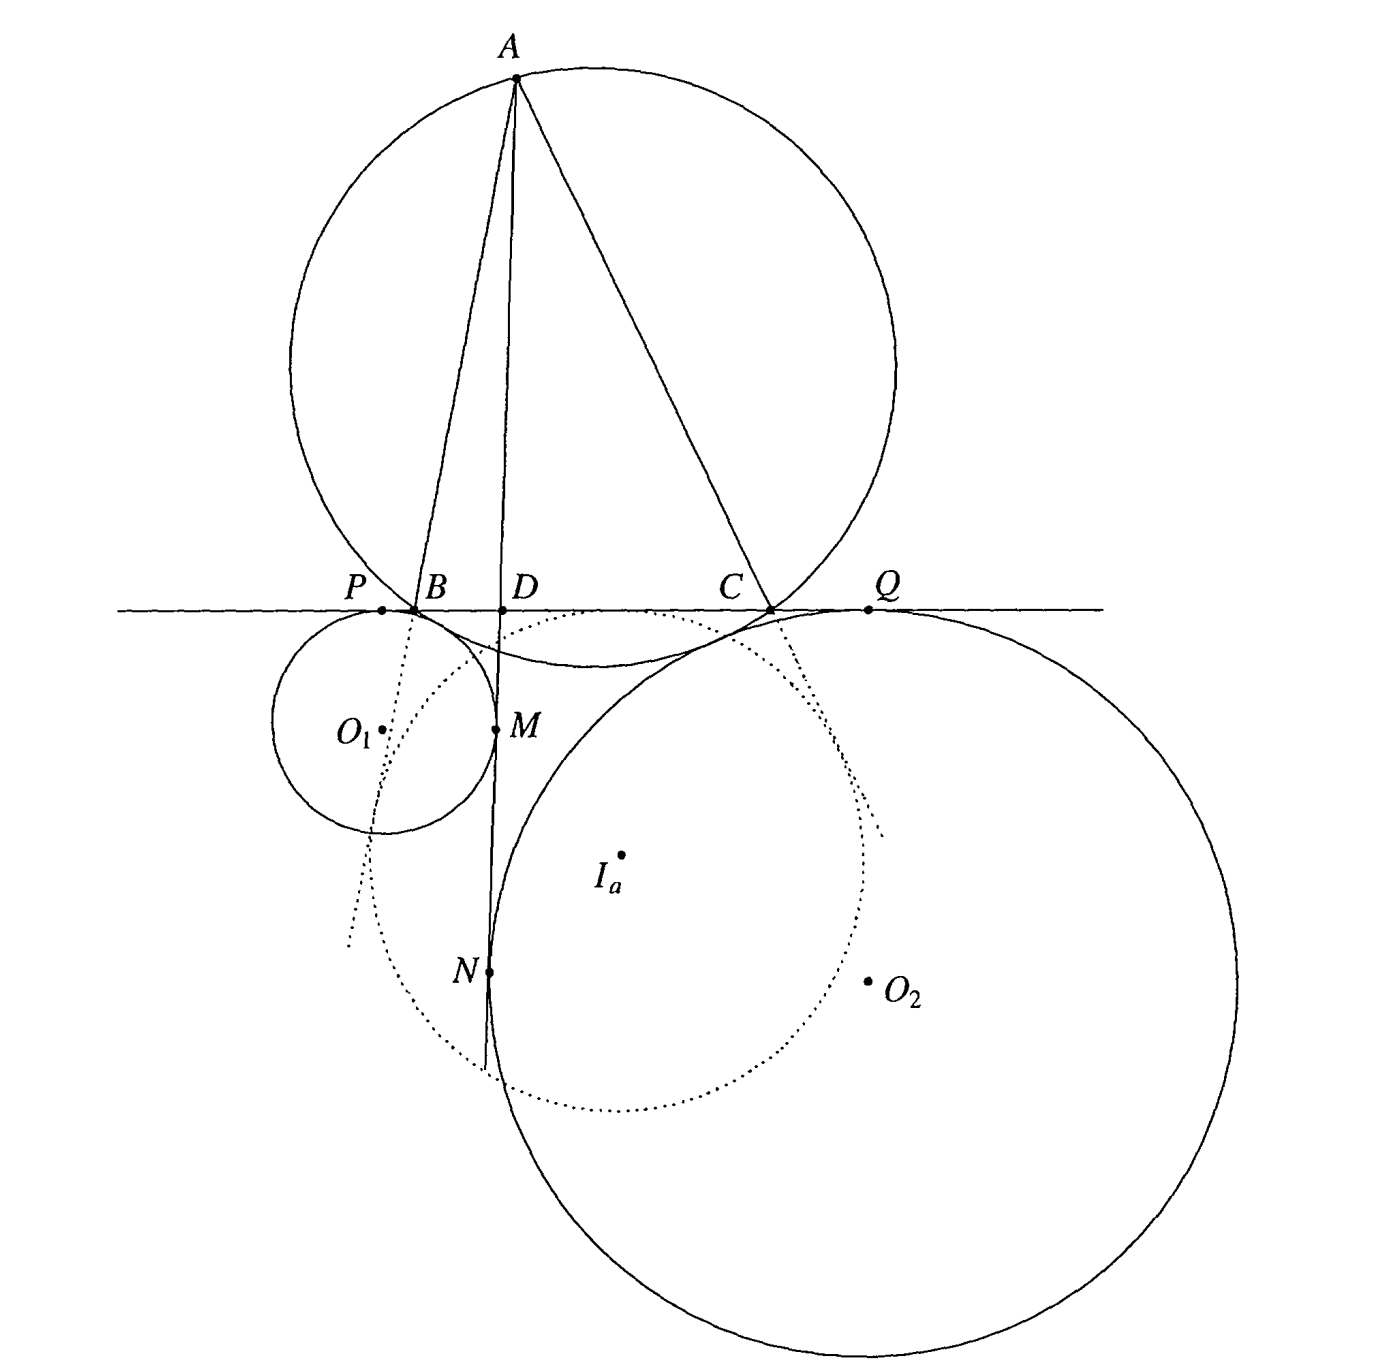
\includegraphics[width=0.8\linewidth]{Эльзята/Яма/16.pics/pic_1.png}
    \caption{}
    \label{fig:placeholder}
\end{figure}